%%%% I-POMCP: IJCAI-27 submission

\documentclass{article}
\pdfpagewidth=8.5in
\pdfpageheight=11in

\usepackage{ijcai27}

\usepackage{times}
\usepackage{soul}
\usepackage{url}
\usepackage[hidelinks]{hyperref}
\usepackage[utf8]{inputenc}
\usepackage[small]{caption}
\usepackage{graphicx}
\usepackage{amsmath}
\usepackage{amssymb}
\usepackage{amsthm}
\usepackage{booktabs}
\usepackage{algorithm}
\usepackage{algorithmic}
\usepackage{tikz}
\usetikzlibrary{arrows.meta,positioning,fit,calc}
\usepackage[switch]{lineno}

% Comment out this line in the camera-ready submission
\linenumbers

\urlstyle{same}

\newtheorem{definition}{Definition}
\newtheorem{proposition}{Proposition}

% Notation of Gmytrasiewicz and Doshi (2005)
\newcommand{\IS}{\mathit{IS}}
\newcommand{\SE}{\mathit{SE}}
\newcommand{\ER}{\mathit{ER}}
\newcommand{\OPT}{\mathit{OPT}}
\newcommand{\SEN}{\widetilde{\SE}^{N}}
\newcommand{\hth}{\hat{\theta}}
\renewcommand{\Pr}{\mathit{Pr}}
% Textual citations with the named style
\newcommand{\citet}[1]{\citeauthor{#1}~\shortcite{#1}}
\newcommand{\todo}[1]{\textcolor{red}{[TODO: #1]}}

\pdfinfo{
/TemplateVersion (IJCAI.2027.0)
}

\title{Interactive POMCP: Online Monte Carlo Planning\\in Finitely Nested I-POMDPs}

\author{
    Anonymous Submission
}

\begin{document}

\maketitle

\begin{abstract}
Interactive POMDPs let an agent plan in the presence of other agents by maintaining beliefs over the physical state and over models of the other agents, including their beliefs. Exact solutions are out of reach beyond small problems, and the online planners used in practice represent nested beliefs by sampled particles, which misjudge modeled agents near their decision thresholds and break down under deterministic observations. We present Interactive POMCP (I-POMCP), an online Monte Carlo tree search planner for finitely nested I-POMDPs whose nested beliefs are exact or compressed from exact updates, and whose search values are rescored with the exact observation law, yielding certified per-action value intervals. In three domains and at nesting levels up to 4, I-POMCP makes Bayes-optimal decisions at beliefs reachable from the common prior, where the interactive particle filter and nested Monte Carlo tree search reach at most 81\% of them at any budget we tried; it remains well defined under deterministic observations where sampled filters fail; and its exact counterpart shows when one more level of reasoning pays: against an agent whose actions depend on its beliefs about the planner, while against one whose actions do not, it costs.
\end{abstract}

%======================================================================
\section{Introduction}
\label{sec:intro}

An agent that shares its environment with other rational agents must predict their actions, which depend on what they believe, including what they believe about the agent itself. Interactive POMDPs (I-POMDPs) \cite{gmytrasiewicz2005framework} formalize this from the point of view of an individual agent, replacing the beliefs over physical states of POMDPs \cite{kaelbling1998planning} with beliefs over interactive states, which combine the physical state with models of the other agents. Intentional models ascribe beliefs, preferences and rationality to the other agent, so the beliefs nest; finitely nested I-POMDPs bound the nesting at a strategy level $l$.

The price of this expressiveness is computational. Each update of a level-$l$ belief must anticipate every action and observation of the other agent and update its level-$(l-1)$ belief accordingly, and each anticipated action is itself the solution of the other agent's problem one level down. Exact solutions are therefore limited to small problems and short horizons \cite{rathnasabapathy2006exact}, and practice relies on sampling: interactive particle filters with reachability-tree sampling \cite{doshi2009monte}, adaptations of POMCP \cite{silver2010monte} to I-POMDPs \cite{hula2015monte}, and nested Monte Carlo tree search \cite{schwartz2022online}. Sampled nested beliefs are brittle: a modeled agent close to a decision threshold can be predicted to take the wrong action, and under deterministic observations every particle can contradict what the agent perceives, leaving the update undefined.

In this paper we take a different route: the planner computes nested beliefs and the quantities its search integrates exactly wherever this is affordable, and approximates only where it is not. Our contributions are as follows.
\begin{enumerate}
    \item \textbf{I-POMCP}, an online planner for finitely nested I-POMDPs (Section~\ref{sec:method}). It searches over the agent's own observation histories, carries its interactive belief down the tree, and integrates immediate rewards and last-step values exactly. Nested beliefs are held exactly, or compressed from exact updates beyond a bound $N$. After search, the tree is rescored with the exact observation law, which yields certified intervals on the action values at every decision.
    \item \textbf{Near-tie escalation} (Section~\ref{sec:escalation}): the planner's own gap between its two best action values identifies the decisions that belief compression can change, and only those are re-decided with a larger belief bound.
    \item \textbf{An evaluation across three domains and nesting levels 0--4} (Section~\ref{sec:results}): two versions of the multi-agent tiger game, UAV reconnaissance and a two-agent Wumpus world; the computation the interactive particle filter, nested Monte Carlo tree search and I-POMCP need to reach the Bayes-optimal decision; and an analysis, by proposition (Section~\ref{sec:depth}), with zero-variance exact values and in paired episodes, of when an additional level of reasoning pays and when it costs.
\end{enumerate}

%======================================================================
\section{Background: Finitely Nested I-POMDPs}
\label{sec:background}

We follow the notation of \citet{gmytrasiewicz2005framework}. For simplicity of presentation we consider an agent $i$ interacting with one other agent, $j$.

\begin{definition}[I-POMDP]
An interactive POMDP of agent $i$ is $\text{I-POMDP}_i = \langle \IS_i, A, T_i, \Omega_i, O_i, R_i \rangle$, where $\IS_i = S \times M_j$ is the set of interactive states, $S$ is the set of physical states and $M_j$ the set of models of agent $j$; $A = A_i \times A_j$ is the set of joint actions; $T_i : S \times A \times S \to [0,1]$ is the transition function; $\Omega_i$ is the set of $i$'s observations and $O_i : S \times A \times \Omega_i \to [0,1]$ its observation function; and $R_i : \IS_i \times A \to \mathbb{R}$ is $i$'s reward function.
\end{definition}

The forms of $T_i$ and $O_i$ reflect the assumptions that agents' actions do not change the other agents' models directly, and that agents cannot observe each other's models. An intentional model of $j$ is a type $\theta_j = \langle b_j, \hth_j \rangle$, consisting of $j$'s belief $b_j$ and its frame $\hth_j = \langle A_j, \Omega_j, T_j, O_j, R_j, OC_j \rangle$. Subintentional models, $SM_j$, are simpler; the no-information model, which assigns equal probability to each of $j$'s actions, is one of them.

\paragraph{Finite nesting.} Finitely nested I-POMDPs are constructed bottom-up:
\begin{align*}
\IS_{i,0} &= S, & M_{j,0} &= \Theta_{j,0} \cup SM_j,\\
\IS_{i,l} &= S \times M_{j,l-1}, & M_{j,l} &= \Theta_{j,l} \cup M_{j,l-1},
\end{align*}
where $\Theta_{j,l} = \{\langle b_{j,l}, \hth_j \rangle : b_{j,l} \in \Delta(\IS_{j,l})\}$. The parameter $l$ is the strategy level. Since $M_{j,l-1}$ contains the models of all lower levels, a level-$l$ agent may be uncertain about the other agent's level as well as its beliefs. Level-0 agents follow the no-information model, and the frames are common knowledge.

\paragraph{Belief update.} After action $a_i^{t-1}$ and observation $o_i^t$, $i$'s new belief, $b_i^t = \SE_{\theta_i}(b_i^{t-1}, a_i^{t-1}, o_i^t)$, is \cite{gmytrasiewicz2005framework}:
\begin{multline}
b_i^t(is^t) = \beta \!\!\sum_{is^{t-1}:\, \hth_j^{t-1} = \hth_j^t}\!\! b_i^{t-1}(is^{t-1}) \sum_{a_j^{t-1}} \Pr(a_j^{t-1} \mid \theta_j^{t-1})\\
\times O_i(s^t, a^{t-1}, o_i^t)\, T_i(s^{t-1}, a^{t-1}, s^t) \sum_{o_j^t} O_j(s^t, a^{t-1}, o_j^t)\\
\times \tau_{\theta_j^t}(b_j^{t-1}, a_j^{t-1}, o_j^t, b_j^t),
\label{eq:update}
\end{multline}
where $\beta$ is a normalizing constant, $\tau_{\theta_j^t}(b_j^{t-1}, a_j^{t-1}, o_j^t, b_j^t)$ is 1 if $b_j^t = \SE_{\theta_j}(b_j^{t-1}, a_j^{t-1}, o_j^t)$ and 0 otherwise, and $\Pr(a_j \mid \theta_j) = 1/|\OPT(\theta_j)|$ if $a_j \in \OPT(\theta_j)$ and 0 otherwise. For a level-0 model, $\Pr(a_j \mid \theta_j) = 1/|A_j|$ and the model does not change. The recursion in $\OPT(\theta_j)$ and in $\SE_{\theta_j}$ terminates at level 0.

\paragraph{Values and solutions.} With $H$ steps to go and discount factor $\gamma$, the value of $\theta_i = \langle b_i, \hth_i \rangle$ is $U^H(\theta_i) = \max_{a_i \in A_i} Q^H(\theta_i, a_i)$, where
\begin{multline}
Q^H(\theta_i, a_i) = \sum_{is} \ER_i(is, a_i)\, b_i(is)\\
+ \gamma \sum_{o_i \in \Omega_i} \Pr(o_i \mid a_i, b_i)\, U^{H-1}\big(\langle \SE_{\theta_i}(b_i, a_i, o_i), \hth_i \rangle\big),
\label{eq:value}
\end{multline}
$\ER_i(is, a_i) = \sum_{a_j} R_i(is, a_i, a_j) \Pr(a_j \mid m_j)$, and $U^0 \equiv 0$. The optimal actions $\OPT(\theta_i)$ are the maximizers of Eq.~\ref{eq:value}.

%======================================================================
\section{Related Work}
\label{sec:related}

\paragraph{Exact and offline solutions.} Exact solutions group the other agent's models into behaviorally equivalent classes \cite{rathnasabapathy2006exact}. Offline approximations include interactive point-based value iteration \cite{doshi2008generalized}, interactive bounded policy iteration \cite{sonu2015scalable}, and interactive dynamic influence diagrams solved with model equivalences \cite{zeng2012exploiting}. Recursive modeling \cite{gmytrasiewicz2000rational} and the cognitive hierarchy model \cite{camerer2004cognitive} motivate uncertainty over the other agent's level.

\paragraph{Online planning.} The interactive particle filter \cite{doshi2009monte} represents the belief at each nesting level by $N$ particles weighted by the observation likelihood, and reachability-tree sampling (RTS) looks ahead by expanding $K$ sampled observations per node; together they are the standard approximation and our first baseline. I-POMDP Lite \cite{hoang2013interactive} assumes that the other agent observes the physical state, so it cannot represent that agent's beliefs about the planner. \citet{hula2015monte} adapted POMCP to I-POMDPs to explain human play in a trust game. I-NTMCP \cite{schwartz2022online}, our second baseline, builds one Monte Carlo search tree per nesting level over particles of states and histories, and needs only a generative model. POTMMCP \cite{schwartz2023combining} plans against a finite set of fixed policies rather than against agents that model the planner, and IPOMDP-Net \cite{han2019ipomdpnet} learns an I-POMDP model and plans with a QMDP approximation.

\paragraph{What is new.} To our knowledge, no prior I-POMDP planner holds nested beliefs as exact updates with bounded compression, provides certified bounds on its action values, or maintains uncertainty over the other agent's level jointly with its nested beliefs.

%======================================================================
\section{Interactive POMCP}
\label{sec:method}

I-POMCP is an online planner: at every step it plans from agent $i$'s current interactive belief with a fixed lookahead $H$, executes the chosen action, and updates the belief with the observation it receives. Its components are a compressed interactive belief filter (Section~\ref{sec:filter}), a Monte Carlo tree search over $i$'s private histories (Section~\ref{sec:search}), exact rescoring of the finished tree with certified intervals (Section~\ref{sec:scoring}), and recursive solutions of the other agent's models (Section~\ref{sec:modeled}).


%----------------------------------------------------------------------
\subsection{Compressed Interactive Belief Filter}
\label{sec:filter}

The update in Eq.~\ref{eq:update} can be computed exactly when the belief has finite support, by enumerating the support of $b_i^{t-1}$, the actions of $j$ with positive probability under each model, the next physical states and $j$'s observations, and merging interactive states that coincide; representing every belief, at every level, as a sorted list of atoms gives the canonical form that merging requires. The difficulty is size: the support may multiply by up to $|A_j|\,|\Omega_j|$ at every step and at every level of nesting.

\begin{definition}[Compressed update]
Given a bound $N$, the compressed update $\SEN_{\theta_i}(b_i, a_i, o_i)$ computes the exact update of Eq.~\ref{eq:update}, in which every nested model $\theta_j$ is advanced by its own compressed update $\SEN_{\theta_j}$, and then, only if the posterior has more than $N$ distinct atoms, replaces it by $N$ stratified draws \cite{douc2005comparison} taken in canonical order, merging duplicates.
\end{definition}

The compressed update has three properties that matter for planning. A belief whose support stays within $N$ atoms is updated exactly; the evidence $\Pr(o_i \mid a_i, b_i)$ is computed exactly under the compressed prior, so a possible observation is never assigned zero probability, even under deterministic sensors; and the compression error per atom is below $1/N$, and occurs only where the support exceeds the bound. The interactive particle filter \cite{doshi2009monte}, by contrast, samples every term of every update. The supplement gives the update and the recursive solution of the other agent's models as pseudocode.

%----------------------------------------------------------------------
\subsection{Search over Private Histories}
\label{sec:search}

I-POMCP estimates $Q^H(\theta_i, a_i)$ of Eq.~\ref{eq:value} by Monte Carlo tree search \cite{kocsis2006bandit,silver2010monte} over $i$'s private histories $h$, i.e., sequences of $i$'s own actions and observations since the current step (Algorithm~\ref{alg:search}). Unlike POMCP, every node carries $i$'s interactive belief $b_h$, obtained from its parent's belief with the same compressed update used for real observations. Each simulation descends the tree; at history $h$ with $r$ steps to go it selects an action by the upper confidence bound
\begin{equation}
a_i = \arg\max_{a} \Big[ Q(h, a) + c\, W_r \sqrt{\log N(h) / N(h, a)} \Big],
\label{eq:ucb}
\end{equation}
where $W_r = (R_{\max} - R_{\min}) \sum_{t < r} \gamma^t$ is the range of an $r$-step discounted return, computed from the declared bounds of $R_i$, and $c$ is a dimensionless constant. It then draws an interactive state $(s, \theta_j)$ from $b_h$, obtains $j$'s action from the solution of $\theta_j$ (Section~\ref{sec:modeled}), and samples the next physical state and $i$'s observation. Drawing the interactive state from $b_h$ at every step makes the observation distribution in the tree equal to $\Pr(o_i \mid a_i, b_h)$, which the backup integrates.

Two quantities are integrated exactly rather than sampled: the immediate reward $\ER_i(b_h, a_i) = \sum_{is} \ER_i(is, a_i)\, b_h(is)$ at every history, and the value $\max_{a_i} \ER_i(b_h, a_i)$ of the last decision ($r = 1$), the boundary condition of Eq.~\ref{eq:value}. This removes the variance of sampled rewards from the backups without using information that $i$ does not have. A new child is valued by one rollout of a domain policy that depends only on $i$'s observations, and backups are weighted by the observation counts $C(h, a, o)$:
\begin{equation}
Q(h, a) = \ER_i(b_h, a) + \gamma \sum_{o} \frac{C(h, a, o)}{N(h, a)}\, V(h a o),
\label{eq:backup}
\end{equation}
where $V(h) = \max_a Q(h, a)$ over the actions evaluated at $h$, and a simulated step that ends the episode contributes zero continuation.

\begin{algorithm}[t]
\caption{I-POMCP decision of agent $i$}
\label{alg:search}
\textbf{Input}: belief $b_i$, frame $\hth_i$, lookahead $H$, simulations $n$\\
\textbf{Output}: action, scored values $Q^\star$, intervals $[Q^-, Q^+]$
\begin{algorithmic}[1]
\STATE create root history $\emptyset$ with $b_\emptyset \leftarrow b_i$
\FOR{$k = 1, \ldots, n$}
    \STATE \textsc{Simulate}$(\emptyset, H)$
\ENDFOR
\STATE $(Q^\star, Q^-, Q^+) \leftarrow$ \textsc{Score}$(\emptyset, H)$ \hfill (Section~\ref{sec:scoring})
\STATE \textbf{return} $a \in \arg\max_{a} Q^\star(\emptyset, a)$, uniformly over ties
\STATE
\STATE \textbf{procedure} \textsc{Simulate}$(h, r)$
\IF{$r = 1$}
    \STATE \textbf{return} $\max_{a} \ER_i(b_h, a)$
\ENDIF
\STATE choose $a_i$ by Eq.~\ref{eq:ucb}
\STATE draw $(s, \theta_j) \sim b_h$; $a_j \sim \Pr(\cdot \mid \theta_j)$ \hfill (Sec.~\ref{sec:modeled})
\STATE draw $s' \sim T_i(s, \langle a_i, a_j \rangle, \cdot)$, $o_i \sim O_i(s', \langle a_i, a_j \rangle, \cdot)$
\IF{$h a_i o_i$ is not in the tree}
    \STATE add $h a_i o_i$ with $b_{h a_i o_i} \leftarrow \SEN_{\theta_i}(b_h, a_i, o_i)$
    \STATE $v \leftarrow$ \textsc{Rollout}$(h a_i o_i, r - 1)$
\ELSE
    \STATE $v \leftarrow$ \textsc{Simulate}$(h a_i o_i, r - 1)$
\ENDIF
\STATE increment $N(h)$, $N(h, a_i)$, $C(h, a_i, o_i)$; update $Q(h, a_i)$ by Eq.~\ref{eq:backup}
\STATE \textbf{return} $Q(h, a_i)$
\end{algorithmic}
\end{algorithm}

%----------------------------------------------------------------------
\subsection{Exact Chance Scoring and Certified Intervals}
\label{sec:scoring}

After the simulations, the finished tree is rescored bottom-up with the exact observation law in place of the sampled frequencies:
\begin{equation}
Q^\star(h, a) = \ER_i(b_h, a) + \gamma \sum_{o} \Pr(o \mid a, b_h)\, V^\star(h a o),
\label{eq:score}
\end{equation}
where the sum ranges over observations of positive probability, $V^\star(h) = \max_a Q^\star(h, a)$ over the evaluated actions, and $V^\star = \max_a \ER_i(b_h, a)$ at the last decision. With two steps to go, every child is a last decision whose exact value needs only its belief, so the action is scored over all of its positive observation branches, sampled or not; with more steps to go, an action with an unsampled observation of positive probability keeps its search value.

\begin{proposition}[Exact scoring]
\label{prop:exact}
If, at every history of the tree with at least two steps to go, every action of $i$ has been evaluated and every observation of positive probability has a child, then $Q^\star(\emptyset, a) = Q^H(\langle b_i, \hth_i \rangle, a)$ for every $a \in A_i$, where $Q^H$ is computed with the other agent's models solved as in Section~\ref{sec:modeled} and with the compressed update.
\end{proposition}
\begin{proof}[Proof sketch]
By induction on the steps to go. At $r = 1$, $V^\star(h) = \max_a \ER_i(b_h, a) = U^1$. If $V^\star(h a o) = U^{r-1}$ for every positive branch, Eq.~\ref{eq:score} equals Eq.~\ref{eq:value} at $b_h$, since $\Pr(o \mid a, b_h)$ and $\ER_i(b_h, a)$ are exact under $b_h$, and the maximum ranges over all of $A_i$.
\end{proof}

The planner records whether the condition of Proposition~\ref{prop:exact} held, propagating it from the leaves. When it does not, the same pass returns certified intervals. Let $\ell_0 = u_0 = 0$ and, for $r \geq 1$, $\ell_r = R_{\min} + \gamma \min(0, \ell_{r-1})$ and $u_r = R_{\max} + \gamma \max(0, u_{r-1})$; these bound any $r$-step return, including returns of episodes that end early. In the computation of $Q^-$ and $Q^+$, exact terms enter exactly, a rollout frontier with $r$ steps to go enters as $[\ell_r, u_r]$, an unsampled observation branch of probability $p$ enters as $p\,[\ell_{r-1}, u_{r-1}]$, and an action never tried enters as $\ER_i(b_h, a) + \gamma\,[\ell_{r-1}, u_{r-1}]$.

\begin{proposition}[Certified intervals]
\label{prop:bounds}
For every $a \in A_i$, $Q^-(\emptyset, a) \leq Q^H(\langle b_i, \hth_i \rangle, a) \leq Q^+(\emptyset, a)$, where $Q^H$ is as in Proposition~\ref{prop:exact}.
\end{proposition}
\begin{proof}[Proof sketch]
By the same induction: every term of Eq.~\ref{eq:value} is either computed exactly or replaced by an interval that contains it, and the maximum of intervals contains the maximum of their members.
\end{proof}

The width of the interval measures the search error that the tree leaves unresolved. It does not account for error in the other agent's model or for compression of the belief.

%----------------------------------------------------------------------
\subsection{Solving the Other Agent's Models}
\label{sec:modeled}

The probability $\Pr(a_j \mid \theta_j)$ in Eq.~\ref{eq:update} and in the search requires $\OPT(\theta_j)$, i.e., the solution of $j$'s own I-POMDP at level $l-1$. I-POMCP obtains it by running I-POMCP for $j$ at $b_j$, with a separate simulation budget for modeled agents and with $j$'s models of $i$ solved one level further down, until level 0 is reached. The modeled agent acts uniformly over the maximizers of its scored values, so it is predicted by the same rule by which $i$ itself decides; when the scores are exact, values within a relative $10^{-9}$ are tied, as in the exact solution.

Every solve is seeded from a canonical digest of the modeled belief and the configuration, so a modeled policy is a deterministic function of the model, and solutions are cached across searches and real steps. The modeled budget is adaptive: a modeled solve grows one tree by doubling and stops once the gap between its two leading actions exceeds a Bonferroni-corrected $t$ critical value times the spread of a few independent pilot trees; at its cap it equals a flat search.

Finally, every prior over levels keeps positive probability on level 0. Under deterministic observations, a modeled $j$ whose model of $i$ is concentrated on one level can receive an observation that this model deems impossible; since the no-information model gives every action positive probability, level-0 mass keeps $\SE_{\theta_j}$ defined whenever the observation is possible at all.

%----------------------------------------------------------------------
\subsection{Near-Tie Escalation}
\label{sec:escalation}

Compression with a small bound $N$ can change a decision only where the decision is close, and the planner measures closeness itself, by the gap between its two largest scored values. Each agent at level 2 or higher keeps a \emph{shadow}: the same planner, with the same seeds, at a larger bound $N' > N$, conditioned on the same realized actions and observations. When the base planner's top-two gap is at most a threshold $g$, the shadow decides; otherwise the base decision stands. Modeled agents are solved by the base planner only. We use $N = 64$, $N' = 1{,}024$ at level 2 and 256 at levels 3--4, and $g = 3$ in reward units.

%======================================================================
\section{When Does a Deeper Model Pay?}
\label{sec:depth}

A higher strategy level is more expensive; when is it worth its cost? Fix the real agent $j$ and the lookahead $H$. We call two models of $j$ \emph{predictively equivalent} at a history of $i$ when they induce the same joint distribution over the next $H$ steps of $j$'s actions and $i$'s observations.

\begin{proposition}[Correct prediction suffices]
\label{prop:prediction}
If $i$'s model of $j$ is predictively equivalent to the real $j$ at every history of the next $H$ steps, then $i$'s exact solution maximizes $i$'s true expected $H$-step reward at the current decision, and no other model of $j$, of any level or prior, does better at that decision.
\end{proposition}
\begin{proof}
Given the predictive distribution, $i$'s planning problem is a POMDP over the physical state and $j$'s internal state, whose transition and observation functions are fixed by that distribution. Predictively equivalent models induce the same POMDP and hence the same $Q^H$, which the exact solution maximizes.
\end{proof}

In particular, if $j$'s actions do not depend on any belief about $i$, as for the no-information model, a level-1 agent that models $j$ correctly is already optimal, and a deeper agent gains nothing at that decision and may lose. An additional level can pay only when the real agent's actions depend on its beliefs about $i$, and only when the payoffs make $i$'s best response sensitive to those actions. The proposition concerns a single decision; receding-horizon episodes carry no such guarantee, so we test it empirically (Section~\ref{sec:depth-results}).

%======================================================================
\section{Experimental Setup}
\label{sec:setup}

\subsection{Domains}

All three domains are two-agent and finite, with explicit transition, observation and reward functions, which both the planner and the exact references require.

\paragraph{Multi-agent tiger.} Two agents face two doors, one hiding a tiger and the other a prize \cite{gmytrasiewicz2005framework}, so there are two physical states. Each agent can listen or open a door; listening costs 1, opening the tiger's door costs 100 and opening the other door pays 10, and if either agent opens a door the tiger is placed at random. A listening agent hears the tiger's growl from the correct side with probability 0.85, together with a creak that reports the other agent's action with probability 0.9. In this game, which we call the \emph{original} game, each agent's payoff depends only on its own door. We also use a \emph{coordination} variant with the same states, transitions and observations, in which each agent's payoff depends on the other agent's action: an agent that opens the safe door in the same step as the other agent receives 40 instead of 10. The joint payoff was chosen so that the exact value of one more level of reasoning is positive at reachable beliefs. We use the original game only for single decisions and the comparison with the baselines; all results on levels and depth use the coordination game, UAV reconnaissance and the Wumpus world.

\paragraph{UAV reconnaissance and the Wumpus world.} In UAV reconnaissance \cite{doshi2009monte}, an unmanned aerial vehicle $i$ seeks a ground target $j$ on a $3 \times 3$ grid of sectors (81 physical states, 5 actions per agent). The UAV receives 50 for spotting the target, which ends the episode, and pays 5 for every other step; the target loses 50 when spotted. Parameters the original description leaves open follow \citet{zeng2012exploiting}. In the two-agent Wumpus world, a human $i$ searches a $3 \times 3$ grid with one pit for gold, while a wumpus $j$ hunts the human (2{,}048 initial states). The human receives 1000 for the gold and $-1000$ for dying, and the wumpus 1000 for catching the human and $-1000$ for being shot; every other step costs 1. All percepts are deterministic, which makes this domain a stress test for sampled beliefs. The supplement specifies both domains in full.

\subsection{Exact References}

\paragraph{Decisions.} For a single decision, we solve the finite-horizon I-POMDP of Eq.~\ref{eq:value} by full enumeration, with exact beliefs and every lower level solved exactly in turn; a modeled agent with several optimal actions plays them uniformly. A decision with policy $\pi$ at belief $b_i$ is scored by its first-action loss, $U^H(\theta_i) - \sum_{a} \pi(a)\, Q^H(\theta_i, a)$, the value it loses if every later decision is optimal. A decision is \emph{optimal} when its loss is at most $10^{-9}$.

\paragraph{Episodes.} Each agent's realized actions and observations are replayed through the \emph{exact} (Bayes-optimal) agent of the same level, with the same frames, level priors and lookahead, exact beliefs, and every level solved exactly. At every step we test whether the agent's action is optimal for the exact agent, and compare the two posteriors over the other agent's level by total variation. Exact beliefs grow about threefold per step, so the replay covers an \emph{exact window} of 10, 8, 4 and 3 steps at levels 1--4 in the tiger game, and 20 and 10 steps at levels 1 and 2 in UAV reconnaissance. Inside the window, the expected reward of a pair of exact agents is computed with zero variance by enumerating the joint process of the physical state and both agents' beliefs.

\subsection{Baselines}

\paragraph{IPF + RTS.} The interactive particle filter with reachability-tree sampling \cite{doshi2009monte} uses $N = 64$ particles at every level and $K \in \{2, 4, 8\}$ sampled observations per node. We run it both plain and with likelihood smoothing, in which each particle is weighted by $(1-\epsilon) O_i + \epsilon / |\Omega_i|$ with $\epsilon = 0.01$, the standard repair for particles of zero likelihood.

\paragraph{I-NTMCP.} We run the authors' implementation of \citet{schwartz2022online}, unchanged, through an adapter to our domains, with their default parameters, our level $l$ as their nesting level $l-1$, and $M$ simulations per search. We run the released code and a variant that after each real step reinvigorates particles from our exact transition and observation functions, and report the stronger of the two at each budget. On the authors' own domain, their runner reproduces their published results exactly and the adapter matches them, at 1.45 times the CPU per search (supplement).

All planners are implemented in Python and run single-threaded, one process per decision, and we report process CPU time per decision, nested solves included.

\subsection{Protocols and Measures}

\paragraph{Decisions at reachable beliefs.} To compare the planners on beliefs that agents reach in play, and on problems that every planner can take (I-NTMCP requires a common prior), we generate agent $i$'s histories from the common prior: $i$ acts uniformly at random among the actions that do not end the episode, and $j$ acts as the exact I-POMDP's own model of it. After 1--5 steps in UAV reconnaissance and 2--4 steps in the Wumpus world, the exact I-POMDP of level 2, with $j$ at level 1, is solved at $i$'s belief, and every planner decides the same problem. Histories that lead to the same belief are counted once: 512 distinct beliefs in UAV reconnaissance and 219 in the Wumpus world, of which a fixed random subset of 100 is decided by every planner and budget. No budget was chosen on these beliefs. Planners are compared with exact McNemar tests \cite{mcnemar1947note}, Holm-corrected \cite{holm1979simple}.

\paragraph{Decisions at chosen beliefs.} I-POMCP's budgets were chosen on grids of named beliefs at levels 1--4 and horizons 2--5, in which $i$'s and $j$'s beliefs about the physical state are crossed (supplement), and tested, unchanged, on random beliefs and seeds that the selection did not use.

\paragraph{Episodes.} In the coordination tiger game, agent $i$ at levels 0--4 plays $j$ at levels 0--4 in 10-step episodes, with $H = 2$, $\gamma = 0.95$, 100 simulations, $N = 64$, and a uniform prior over the other agent's lower levels at every level of nesting. The game is symmetric, so the cells with $i$'s level at least $j$'s determine the grid; we run $n = 15{,}000$ episodes per cell at levels up to 2, 700 when $i$ is at level 3, and 100 when $i$ is at level 4, where $n$ is the number of independent episodes. In UAV reconnaissance and the Wumpus world, both agents play at levels 0--2 in 20-step episodes ($n = 100$ per cell), with $H = 3$ and 1{,}000 simulations (UAV) or $H = 2$, 400 simulations and exact beliefs (Wumpus). The primary endpoint is the gain from one more level of $i$ against the same $j$, paired by random seed. Given both agents' actions and observations, the tiger's location follows a hidden Markov model, so each sampled reward of the tiger game is replaced by its exact conditional expectation, computed by forward--backward recursion; the estimand is unchanged and the variance can only decrease \cite{casella1996rao}.

%======================================================================
\section{Results}
\label{sec:results}

\subsection{Compute to the Bayes-Optimal Decision}
\label{sec:compute}

\begin{figure}[t]
\centering
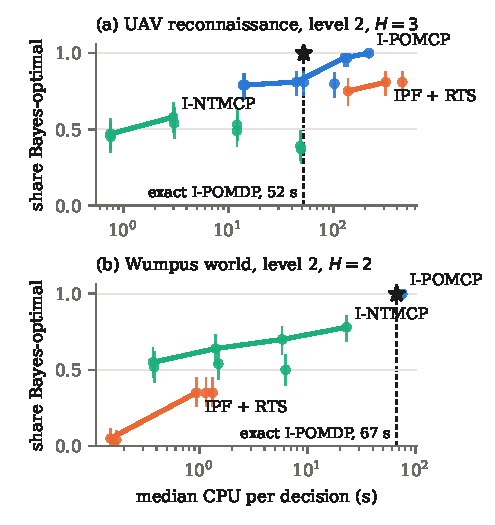
\includegraphics[width=\columnwidth]{compute_benchmark_col.pdf}
\caption{Share of Bayes-optimal decisions at reachable beliefs against median CPU per decision, for every planner and budget on the same 100 distinct beliefs (95\% Clopper--Pearson intervals). Lines join each planner's best share at no more CPU. I-NTMCP's CPU includes the 1.45-fold overhead of our adapter (supplement).}
\label{fig:compute}
\end{figure}

Figure~\ref{fig:compute} shows how much computation each planner needs to decide as the Bayes-optimal agent does. In UAV reconnaissance, I-POMCP reaches the benchmark: with exact beliefs and the target modeled with 1{,}600 simulations, all 100 decisions are optimal (lower bound 0.964) at a median of 217~s. Its rungs are separated by the belief bound, not by simulations. With $N = 64$, root budgets from 100 to 1{,}000 and modeled budgets from 100 to 400 all give 79--81\%, although 89--94\% of the decisions lose at most 0.05; with $N = 1{,}024$ or exact beliefs, 97\%. The misses come from compression inside the search tree, where the support of a belief grows up to 45-fold per simulated step: exact beliefs remove every one we examined, while a 4{,}000-simulation root or a 1{,}600-simulation target at $N = 64$ removes none. IPF + RTS levels off at 75--81\% for $K$ from 2 to 8, at 137--451~s per decision, with losses up to 8.9; I-NTMCP reaches at most 58\%, with losses up to 55, and becomes less accurate with more simulations (37--39\% at $M = 64{,}000$), consistent with its prediction of the target by a softmax over visit counts rather than by the target's best response. On the same beliefs, I-POMCP is right where a baseline is wrong on 19--63 beliefs and never the converse (Holm $p \leq 10^{-5}$ for every baseline and budget).

In the Wumpus world, whose percepts are deterministic, I-POMCP with exact beliefs is optimal on all 219 distinct reachable beliefs (lower bound 0.983) at 75--89~s per decision, already with 100 simulations. The particle filter of IPF + RTS fails on about 90\% of them, because every particle contradicts an observation; likelihood smoothing repairs that case but still fails on about 25\%, where every particle of the wumpus's own belief ends the episode, and the smoothed planner is optimal on 35\%. I-NTMCP improves with $M$ but reaches only 77\% at $M = 64{,}000$, with losses up to 639; on the same beliefs, I-POMCP is never wrong where a baseline is right (Holm $p \leq 10^{-6}$).

At the named beliefs on which its budgets were chosen, I-POMCP is optimal on all 2{,}787 decisions at levels 1--4 and horizons 2--5 in three domains, and on 960 further random beliefs and seeds (supplement); there, IPF + RTS misses 0.5--9\% of the tiger games' decisions and 31--54\% of UAV decisions. Exact scoring carries much of this precision: turning it off at the root changes 34 of 560 UAV decisions from optimal to suboptimal and none the other way (exact McNemar $p = 1.2 \times 10^{-10}$), and the certified intervals of Proposition~\ref{prop:bounds} contained the exact action values in all 1{,}016 decisions in which we checked them.

\begin{figure*}[t]
\centering
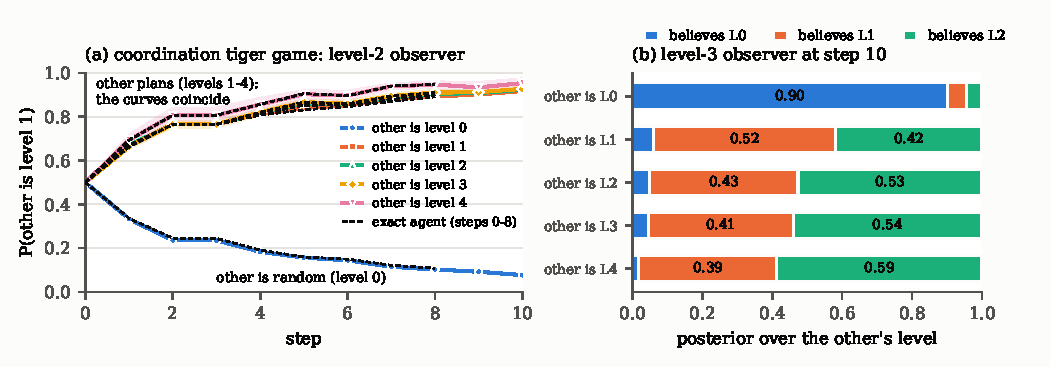
\includegraphics[width=0.86\textwidth]{level_identification.pdf}
\caption{Posteriors over the other agent's level, coordination tiger game. (a) A level-2 observer's probability of level 1, by the other agent's true level (mean and 95\% interval; $n = 15{,}000$ episodes for levels 0--2, 700 for 3, 100 for 4); dashed: the exact observer, steps 0--8 ($n = 1{,}000$, 700, 100). (b) A level-3 observer's posterior at step 10 ($n = 700$; 100 for level 4).}
\label{fig:identification}
\end{figure*}

\subsection{Agents That Act and Infer as the Bayes-Optimal Agent}
\label{sec:episodes}

We replay every agent of the coordination level grid through the exact agent over its exact window. At level 1, every one of 48{,}000 decisions is optimal; at levels 2, 3 and 4, 8{,}779 of 8{,}800, 8{,}361 of 8{,}400 and 1{,}793 of 1{,}800 are (up to 200, 400 and 100 episodes per cell). The other 67 are near-ties (median exact gap 0.09) caused by belief compression at $N = 64$: rebuilt with exact beliefs, each of the 61 we examined chooses an optimal action. Near-tie escalation (Section~\ref{sec:escalation}) removes 32 of 34 such histories on 1{,}600 further episodes and adds none, escalating 3.2\% of the decisions at 0.41 times the CPU of the larger bound throughout. In UAV reconnaissance, all 10{,}391 replayed decisions of both agents at levels 1--2 are optimal. Inside the exact window, the exact pair's expected reward lies within the I-POMCP pair's 95\% interval at 97 of 100 agent-steps of the tiger grid, and at 31 of 36 of the UAV grid; the remaining UAV cases are cells in which all 100 episodes coincide, and one that a fresh sample of 300 episodes resolves (14.3 [10.3, 18.4] against the exact 15.5).

The agents' beliefs about each other are Bayes-exact as well: along the same histories, the exact agent's posterior over the other agent's level (dashed in Figure~\ref{fig:identification}a) coincides with the planner's, with a paired mean difference of at most 0.003 at step 8 in every cell. A level-2 agent comes to believe that the other agent is of level 1 whether it is in fact of level 1, 2, 3 or 4, assigning 0.92--0.95 to level 1 after 10 steps: it can represent only level 0 and level 1, and its posterior concentrates on the hypothesis whose predictions are closest to the truth in Kullback--Leibler divergence \cite{berk1966limiting}, since every planning agent listens until the growls agree and then opens a door. Against an agent that plays at random, the belief in level 1 falls to 0.077 [0.074, 0.080]. A level-3 observer (Figure~\ref{fig:identification}b) separates the levels it can represent: it assigns 0.90 to level 0 when the other agent is random, and its posterior mode is the true level for an agent of level 1 (0.52) or 2 (0.53), while an agent of level 3 or 4 is assigned to its closest model, level 2 (0.54 and 0.59).

\subsection{When One More Level Pays}
\label{sec:depth-results}

\begin{figure}[t]
\centering
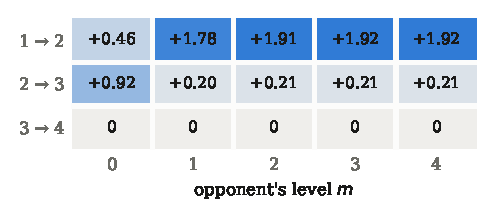
\includegraphics[width=\columnwidth]{level_matchups_col.pdf}
\caption{Exact gain in expected cumulative reward by step 3 from one more level of reasoning, $k \to k + 1$, against an opponent of level $m$, coordination tiger game (exact agents; zero variance).}
\label{fig:matchups}
\end{figure}

Figure~\ref{fig:matchups} gives the value of one more level for exact agents, with zero variance. The second level pays against every intentional opponent (+1.78 to +1.92 by step 3), the third adds about a ninth of that (+0.20 to +0.21), and the fourth adds exactly nothing: a level-4 agent acts as a level-3 agent throughout the window, consistent with 600 fresh episodes of the planner (step 3, $|z| < 1$). I-POMCP's episodes show the same profile at the scale of whole episodes: from level 1 to 2, $i$ gains, by step 10, 7.8 [7.4, 8.3] against $j$ at level 1 ($n = 15{,}000$), 9.2 [7.3, 11.1] against level 3 ($n = 700$) and 7.0 [2.3, 11.8] against level 4 ($n = 100$), while no gain from level 2 to 3 or from 3 to 4 is significant, as expected for a gain of 0.2. The same holds across domains. In UAV reconnaissance, a second level is worth 7.9 by step 8 to the UAV against a level-1 target and 41.3 to the target against a level-1 UAV (exact; in episodes, 6.0 [4.1, 8.2] and 37.5 [33.0, 41.5] over 20 steps), and in the Wumpus world a second level is worth 11.7 to 17.3 by step 5 to the human and 18.9 to 24.6 to the wumpus against an intentional opponent (exact; in episodes, 169 [84, 259] for the human over 20 steps, $n = 200$). A level-2 UAV anticipates a level-1 target's flight to the far corner and spots it after 5.0 steps in every episode, against 6.2 for a level-1 UAV.

\subsection{The Cost of Modeling a Reasoner That Is Not There}
\label{sec:overthinking}

As Proposition~\ref{prop:prediction} implies, a deeper model cannot pay against an opponent whose actions do not depend on its beliefs, and in episodes it costs. Against a random opponent, the exact gain from level 1 to 2 in the coordination game is +0.46 by step 3, $-0.03$ by step 4 and $-0.55$ by step 5, and I-POMCP's episodes lose 0.9 [0.7, 1.1] by step 10: within its lookahead the deeper agent can even gain, since a receding-horizon policy is not optimal for the episode, but its wrong model costs more as the episode continues. In UAV reconnaissance the exact cost is 0.4 to 2.0 for the UAV by steps 5--10 and 1.2 to 3.3 for the target by steps 5--8; over 20-step episodes a level-2 target loses 6.5 [2.0, 11.5] against a random UAV (Holm $p = 0.035$), and a level-2 UAV 5.6 [$-0.4$, 12.0] against a random target, spending moves on a flight that never comes. In the Wumpus world, the second level costs the human 3.4 and the wumpus 1.4 by step 5 against a random opponent (exact; in episodes, 20 [$-70$, 110] for the human). Modeling also has the converse cost of being modeled: a level-1 target, which best-responds to a random UAV, is caught by a level-2 UAV that models exactly that target, and loses 22.7 by step 5 against it, more than a random target would (exact).

%======================================================================
\section{Discussion}
\label{sec:discussion}

The approach has limits. Every result is for two agents, and I-POMCP needs explicit transition, observation and reward functions, while I-NTMCP needs only a generative model. Exact references reach only short horizons, so later decisions in long episodes are judged by reward alone. With a uniform prior over the target's level at $H = 5$, I-POMCP needs a root budget of 64{,}000 to resolve near-ties in UAV reconnaissance, and one decision with a gap of 0.13 stays unresolved there. The budgets we chose at named beliefs do not carry to every reachable belief: at histories of a randomly acting UAV, a belief bound of $N = 64$ makes 79--81\% of decisions Bayes-optimal (89--94\% within 0.05), and exact beliefs are needed for all of them. The Wumpus world at level 2 on a $4 \times 4$ grid is beyond the exact references.

%======================================================================
\section{Conclusion}
\label{sec:conclusion}

I-POMCP holds nested beliefs as exact or compressed updates, integrates rewards and observations exactly where it can, and certifies intervals on its action values. At beliefs that agents reach from the common prior, it makes Bayes-optimal decisions at 75--217~s per decision, where the interactive particle filter and nested Monte Carlo tree search level off at 35--81\% of such decisions at any budget we tried, and its agents act and infer as the Bayes-optimal agent does. One more level of reasoning pays where the other agent's actions depend on its beliefs about the planner. Future work includes equilibrium analysis, more than two agents, and exact scoring with only a generative model.

%======================================================================
\bibliographystyle{named}
\bibliography{references}

\end{document}
